\documentclass[smallextended]{svjour3}
\smartqed
\usepackage{amsmath,amssymb,bm,mathtools}
\usepackage{booktabs,multirow,graphicx}
\usepackage{url}
\usepackage[colorlinks=true,allcolors=blue]{hyperref}
\hypersetup{
  pdftitle={Finite PCG Interpolation Can Outperform the Energy-Minimizing Endpoint in High-Contrast Two-Grid Solvers},
  pdfauthor={Zhengping Cui},
  pdfkeywords={algebraic multigrid, energy-minimizing interpolation, PCG, high-contrast diffusion, two-grid convergence}
}
\emergencystretch=1.5em
\journalname{Journal of Scientific Computing}
\newcommand{\R}{\mathbb{R}}
\newcommand{\T}{\mathsf{T}}
\newcommand{\tr}{\operatorname{tr}}
\newcommand{\diag}{\operatorname{diag}}
\newcommand{\range}{\operatorname{range}}
\newcommand{\supp}{\operatorname{supp}}
\newcommand{\cK}{\mathcal{K}}
\newcommand{\cG}{\mathcal{G}}
\newcommand{\cU}{\mathcal{U}}
\newcommand{\cE}{\mathcal{E}}
\newcommand{\norm}[1]{\lVert#1\rVert}
\newcommand{\abs}[1]{\lvert#1\rvert}
\title{Finite PCG Interpolation Can Outperform the Energy-Minimizing Endpoint in High-Contrast Two-Grid Solvers}
\titlerunning{Finite PCG interpolation for high-contrast two-grid solvers}
\author{Zhengping Cui}
\authorrunning{Z. Cui}
\institute{Z. Cui \at Affiliation and e-mail address to be supplied before submission}
\date{Received: date / Accepted: date}
\begin{document}
\maketitle
\begin{abstract}
Energy minimization is a standard principle for constructing robust algebraic multigrid interpolation. This paper shows that, for a fixed coarse set and smoother, solving the interpolation minimization problem more accurately need not improve the resulting two-grid method. Starting from geometric interpolation, we follow the columnwise Jacobi-preconditioned conjugate-gradient (PCG) path toward the ideal, energy-minimizing endpoint. The interpolation energy decreases strictly at every nonzero step, whereas the true symmetric two-grid spectral radius is generally nonmonotone and may attain a substantially smaller value at an intermediate iterate. We derive an exact graph-space representation of the two-grid objective, identify the unconstrained solver-optimal coarse space, prove convexity of its low sublevel sets, and obtain a singular-value expansion with an explicit second-order remainder near the energy endpoint. This yields two-sided criteria deciding whether an individual PCG step improves or degrades the two-grid spectral radius, together with an arbitrary-path-point certificate. For two-dimensional five-point diffusion, a pinned-capacity estimate gives the sharp scale
$\kappa=\Theta((h^2+[q^2\log(2q)]^{-1})^{-1})$ at bounded contrast, explaining the natural $\Theta(h^{-1})$ PCG scale under fixed physical coarse spacing and the $O(1)$ scale at fixed coarsening ratio. Experiments on high-contrast channelized coefficients verify strict energy decrease, nonmonotone spectral paths, finite graph propagation, robustness over topology, contrast, coefficient seeds and right-hand sides, and a large reduction in both setup density and total solution time. On the central problem, finite PCG reduces 3227 energy-endpoint cycles to 242 and is approximately fifteen times faster in total wall time.
\keywords{algebraic multigrid \and energy-minimizing interpolation \and ideal interpolation \and preconditioned conjugate gradients \and high-contrast diffusion \and two-grid convergence}
\subclass{65F10 \and 65N22 \and 65N55 \and 65F08}
\end{abstract}

\section{Introduction}\label{sec:introduction}
Algebraic multigrid (AMG) succeeds when relaxation and coarse correction divide the error into complementary components. Classical AMG, compatible relaxation, two-grid convergence theory, and modern abstract AMG theory make this principle precise in different ways \cite{ruge1987amg,trottenberg2001multigrid,falgout2005twogrid,brannick2010compatible,xu2017amg}. For difficult high-contrast operators, however, a fixed local geometric interpolation can fail to capture the error left by relaxation. Energy-minimizing interpolation addresses this failure by reducing the energy of the prolongation subject to coarse-variable and near-nullspace constraints \cite{mandel1999energy,wan2000energy,kolev2006energy,brannick2007energy,olson2011energy,brannick2019role,janna2023parallel}.

The established computational interpretation is that an iterative construction may be stopped before the constrained energy problem is solved accurately because a sufficiently good approximation is cheaper and often already effective. We establish a different, stronger phenomenon. Along the same PCG construction path, an inaccurate intermediate iterate may define a \emph{better} coarse space than the accurately computed energy minimizer. Thus finite iteration is not only an economical approximation to a desirable endpoint: it is a regularizing path through a family of competing coarse spaces.

This distinction matters in the regime considered here. We discretize high-contrast diffusion with microstructure near the numerical resolution. On the central $128/16$ cross-channel problem, bilinear interpolation needs 85,524 symmetric two-grid cycles to reduce the residual by $10^{-6}$. The ideal energy-minimizing interpolation is already a strong baseline, reducing this count to 3227. Nevertheless, the finite point $m=43$ on the same Jacobi--PCG path requires only 242 cycles. Hence the improvement is not obtained against a weak geometric baseline: it is a further factor of 13.33 over an endpoint that had already improved the geometric method by a factor of 26.50.

The key reason is geometric. Interpolation energy measures distance to the ideal graph $W^*=-A_{FF}^{-1}A_{FC}$. The two-grid spectral radius instead measures how well the current coarse space captures the image of the fixed smoother. Distance is radial information; the two-grid objective is directional. PCG makes the distance strictly smaller, but its Krylov polynomial can rotate the graph error through directions that alternately help and hurt the smoother-sensitive singular modes.

Our contributions are as follows.
\begin{enumerate}
\item We introduce the normalized graph coordinate $Z=B^{1/2}(W-W^*)S^{-1/2}$. Its singular values are exactly the tangents of the energy principal angles to the ideal coarse space, while the energy gap and Galerkin coarse matrix have exact quadratic forms in $Z$.
\item For the symmetric forward-Gauss--Seidel/coarse/backward-Gauss--Seidel cycle, we prove the exact objective
\begin{equation*}
 \rho_{\rm TG}(Z)=\norm{(I+ZZ^\T)^{-1/2}(T_F-ZT_*)}_2^2.
\end{equation*}
We also identify the best coarse space of a prescribed dimension for the fixed smoother and prove that the low sublevel sets of the corresponding graph objective are convex.
\item Under a simple leading singular value at the endpoint, we derive a first-order expansion with an explicit second-order remainder. The resulting two-sided PCG step criteria rigorously permit both improvement and deterioration despite strict energy decrease. An additional perturbation certificate applies at arbitrary points of the path.
\item We prove finite graph propagation of every column correction. For regular two-dimensional coarse points we obtain a unified boundary--capacity estimate involving
$\Lambda_{h,H}=h^2+[q^2\log(2q)]^{-1}$, $q=H/h$, and prove sharpness separately in the grid and contrast exponents. This explains why $m=\Theta(h^{-1})$ is a natural finite scale under fixed $H$, but not under fixed $q$.
\item Reproducible experiments distinguish the true two-grid spectral radius from right-hand-side-dependent residual factors. They cover 13 cases spanning scale, contrast, and topology; complete paths for two coefficient topologies; fixed-$H$ and fixed-$q$ families; a direct singular-gap diagnostic; five random coefficient seeds; six right-hand sides; repeated timings; and a three-level feasibility study.
\end{enumerate}

Our claims are deliberately separated by level. The algebraic geometry and local perturbation results apply to general symmetric positive definite (SPD) block systems. The capacity and iteration-scale results specialize to regular coarse points for a two-dimensional five-point operator. The multilevel experiment is evidence of transferability, not a multilevel convergence theorem. Related two- and multilevel constructions in a domain-decomposition setting are discussed by Ciaramella and Vanzan \cite{ciaramella2022substructured}; the present mechanism is instead tied to the finite energy-minimization path of interpolation itself.

\section{Model problem and finite energy-minimization path}\label{sec:model}
We consider
\begin{equation}\label{eq:pde}
 -\nabla\!\cdot(a(x)\nabla u)=f\quad\hbox{in }\Omega=(0,1)^2,
 \qquad u=0\quad\hbox{on }\partial\Omega,
\end{equation}
where $0<\alpha\le a(x)\le\beta$ and $\chi=\beta/\alpha\gg1$. A five-point discretization with harmonic face averaging gives an SPD matrix $A$. After a fixed split into fine and coarse variables,
\begin{equation}\label{eq:blockA}
 A=\begin{bmatrix}B&C\\C^\T&A_{CC}\end{bmatrix}\succ0,
 \qquad B=A_{FF}\succ0,
 \qquad P(W)=\begin{bmatrix}W\\I\end{bmatrix}.
\end{equation}
The Galerkin coarse operator is $A_c(W)=P(W)^{\T} A P(W)$. One two-grid cycle consists of one forward Gauss--Seidel sweep, an exact Galerkin coarse correction, and one backward Gauss--Seidel sweep.

The interpolation energy and Schur complement are
\begin{equation}\label{eq:energy-schur}
 J(W)=\frac12\tr(P(W)^{\T} A P(W)),\qquad
 S=A_{CC}-C^{\T}B^{-1}C\succ0.
\end{equation}
The unique energy minimizer is the ideal interpolation block
\begin{equation}\label{eq:ideal}
 W^*=-B^{-1}C.
\end{equation}
Starting from bilinear geometric interpolation $W_0$, we solve every column equation $Bw_j^*=-Ce_j$ by PCG with Jacobi preconditioner $D_B=\diag(B)$. All columns share $B$ and the global step index $m$; a converged column remains fixed. We denote the resulting interpolation by $W_m$ and the high-accuracy endpoint by the condition that every column has relative residual at most $10^{-10}$.

\begin{proposition}[Exact energy identities]\label{prop:energy}
Let $\Delta=W-W^*$. Then
\begin{equation}\label{eq:energy-identities}
 J(W)-J(W^*)=\frac12\norm{\Delta}_{B,F}^2,
 \qquad A_c(W)=S+\Delta^{\T}B\Delta.
\end{equation}
For every PCG step,
\begin{equation}\label{eq:pythagoras}
 \norm{W_m-W^*}_{B,F}^2
 =\norm{W_{m+1}-W^*}_{B,F}^2
 +\norm{W_{m+1}-W_m}_{B,F}^2.
\end{equation}
Consequently every nonzero step strictly decreases $J$.
\end{proposition}
\begin{proof}
Expanding $P(W)^{\T} A P(W)$ and using $BW^*+C=0$ eliminates all terms linear in $\Delta$, giving \eqref{eq:energy-identities}. Columnwise CG Galerkin orthogonality gives
$e_{j,m+1}\perp_B(w_{j,m+1}-w_{j,m})$ with
$e_{j,m}=w_j^*-w_{j,m}$; summing the column Pythagorean identities proves \eqref{eq:pythagoras}.
\end{proof}

Let $\widehat B=D_B^{-1/2}BD_B^{-1/2}$ and
$\widehat e_{j,m}=D_B^{1/2}(w_j^*-w_{j,m})$. Standard CG theory \cite{hestenes1952cg,saad2003iterative} gives
\begin{equation}\label{eq:krylov-poly}
 \widehat e_{j,m}=p_{j,m}(\widehat B)\widehat e_{j,0},
 \quad p_{j,m}(0)=1,
 \quad \deg p_{j,m}\le m,
\end{equation}
and $w_{j,m}$ is the $B$-norm best approximation over its affine Krylov space.

\begin{proposition}[Finite graph propagation]\label{prop:propagation}
Let $\mathcal G_F$ be the graph of the nonzero off-diagonal entries of $\widehat B$, let
$\Omega_j=\supp(\widehat B\widehat e_{j,0})$, and let $\mathcal N_k(\Omega_j)$ be its closed graph-distance-$k$ neighborhood. Then
\begin{equation}\label{eq:finite-propagation}
 \supp(w_{j,m}-w_{j,0})\subseteq\mathcal N_{m-1}(\Omega_j).
\end{equation}
\end{proposition}
\begin{proof}
The correction belongs to
$\operatorname{span}\{\widehat r_{j,0},\widehat B\widehat r_{j,0},\ldots,
\widehat B^{m-1}\widehat r_{j,0}\}$. Multiplication by the sparse graph matrix expands support by at most one edge, and diagonal scaling preserves zero patterns.
\end{proof}

\section{Normalized graph geometry}\label{sec:geometry}
Define
\begin{equation}\label{eq:Z}
 Z=B^{1/2}(W-W^*)S^{-1/2},\quad
 Q_F=\begin{bmatrix}B^{-1/2}\\0\end{bmatrix},\quad
 Q_*=P(W^*)S^{-1/2}.
\end{equation}
The columns of $[Q_F,Q_*]$ form an $A$-orthonormal basis. Direct substitution yields
\begin{align}\label{eq:graph-facts}
 J(W)-J(W^*)&=\frac12\norm{Z}_{F,S}^2,\\
 A_c(W)&=S^{1/2}(I+Z^{\T}Z)S^{1/2},\\
 P(W)&=[Q_F,Q_*]\begin{bmatrix}Z\\I\end{bmatrix}S^{1/2}.
\end{align}
Thus the current energy-coordinate coarse space is the graph
$\cG(Z)=\range[Z^\T,I]^\T$, whereas the endpoint is $\cG(0)$. If the $A$-principal angles to the endpoint are ordered nonincreasingly, then \cite{knyazev2002angles}
\begin{equation}\label{eq:angles}
 \tan\theta_k=\sigma_k(Z).
\end{equation}
Equations \eqref{eq:graph-facts}--\eqref{eq:angles} separate magnitude and direction: the energy controls a weighted Frobenius radius, but not how $Z$ is oriented relative to the smoother.

Let $G$ be the forward Gauss--Seidel error propagator and let the post-smoother be its $A$-adjoint. In energy coordinates set
\begin{equation}\label{eq:T}
 T=A^{1/2}GA^{-1/2},\qquad
 \begin{bmatrix}T_F\\T_*\end{bmatrix}
 =[A^{1/2}Q_F,A^{1/2}Q_*]^\T T.
\end{equation}
Each scalar Gauss--Seidel correction is an $A$-energy projection, so $\norm{T}_2\le1$.

\begin{theorem}[Exact two-grid graph objective]\label{thm:exact-objective}
For exact Galerkin correction and the adjoint smoother pair,
\begin{equation}\label{eq:exact-objective}
 \rho_{\rm TG}(Z)
 =\norm{(I+ZZ^\T)^{-1/2}(T_F-ZT_*)}_2^2.
\end{equation}
\end{theorem}
\begin{proof}
If $\Pi_Z$ is the Euclidean orthogonal projector onto $\cG(Z)$ in energy coordinates, the symmetric two-grid propagator is similar to
$T^\T(I-\Pi_Z)T$. A normalized basis for $\cG(Z)^\perp$ is
\begin{equation*}
 N(Z)=\begin{bmatrix}I\\-Z^\T\end{bmatrix}(I+ZZ^\T)^{-1/2}.
\end{equation*}
Therefore
$\rho_{\rm TG}=\norm{N(Z)^\T[T_F^\T,T_*^\T]^\T}_2^2$, which is \eqref{eq:exact-objective}.
\end{proof}

The endpoint is optimal for $J$, but it need not be optimal for \eqref{eq:exact-objective}. To expose the distinction, consider all $r$-dimensional coarse spaces for a fixed $T$, where $r=n_C$. Write
$T=[U_1,U_2]\diag(\Sigma_1,\Sigma_2)[V_1,V_2]^\T$ with decreasing singular values and $U_1$ containing $r$ columns.

\begin{theorem}[Solver-optimal coarse space]\label{thm:solver-optimal}
For every $r$-dimensional $\cU$,
\begin{equation}\label{eq:solver-lower}
 \rho_{\rm TG}(\cU)\ge\sigma_{r+1}(T)^2,
 \qquad \rho_{\rm TG}(\range(U_1))=\sigma_{r+1}(T)^2.
\end{equation}
For the graph $\cU(X)=\range[I,X^\T]^\T$ in the $[U_1,U_2]$ coordinates,
\begin{equation}\label{eq:optimal-graph}
 \rho_{\rm TG}^{\rm opt}(X)=\lambda_{\max}\!\left[
 (I+XX^\T)^{-1/2}(\Sigma_2^2+X\Sigma_1^2X^\T)
 (I+XX^\T)^{-1/2}\right].
\end{equation}
If $\sigma_r^2>\sigma_{r+1}^2$ and
$\sigma_{r+1}^2<\lambda<\sigma_r^2$, then
\begin{equation}\label{eq:sublevel}
 \{X:\rho_{\rm TG}^{\rm opt}(X)\le\lambda\}
 =\left\{X:\norm{(\lambda I-\Sigma_2^2)^{-1/2}
 X(\Sigma_1^2-\lambda I)^{1/2}}_2\le1\right\}.
\end{equation}
In particular, these sublevel sets are convex, and the objective is nondecreasing along every ray $tX$ as a function of $\abs t$.
\end{theorem}
\begin{proof}
The first statement is the Eckart--Young rank-$r$ lower bound applied to
$(I-\Pi_{\cU})T$. A normalized basis for the complement of $\cU(X)$ gives \eqref{eq:optimal-graph}. The condition
$\rho_{\rm TG}^{\rm opt}(X)\le\lambda$ is equivalent in the Loewner order to
\begin{equation*}
 X(\Sigma_1^2-\lambda I)X^\T\preceq\lambda I-\Sigma_2^2,
\end{equation*}
which is exactly \eqref{eq:sublevel}. Convexity follows because the right-hand side of \eqref{eq:sublevel} is the inverse image of a spectral-norm ball. Radial monotonicity follows by differentiating the associated generalized Rayleigh quotient in $t^2$.
\end{proof}

The theorem gives a fixed-smoother performance baseline independent of energy minimization. It also shows that the solver objective has a well-behaved geometry near its own optimizer. The PCG path, however, is constrained by fixed coarse injection and its Krylov polynomials; it need not point toward that optimizer monotonically.

\section{Why a PCG step may improve or degrade two-grid convergence}\label{sec:local}
Set
\begin{equation}\label{eq:L}
 f(Z)=\sqrt{\rho_{\rm TG}(Z)}=\norm{L(Z)}_2,qquad
 L(Z)=(I+ZZ^\T)^{-1/2}(T_F-ZT_*).
\end{equation}
Assume the leading endpoint singular value is simple:
\begin{equation}\label{eq:gap}
 \sigma=\sigma_1(T_F)>\sigma_2(T_F),\qquad
 \delta=\sigma_1(T_F)-\sigma_2(T_F)>0.
\end{equation}
Let $T_Fv=\sigma u_F$, $T_F^{\T}u_F=\sigma v$, $y=T_*v$, and $\tau=\norm{T_*}_2$. Define, for $z\ge0$,
\begin{equation}\label{eq:eps}
 a(z)=1-(1+z^2)^{-1/2},\quad
 \phi(z)=z(1+z^2)^{-1/2},\quad
 \varepsilon(z)=\sigma a(z)+\tau\phi(z).
\end{equation}

\begin{theorem}[Endpoint expansion with explicit remainder]\label{thm:expansion}
If $z=\norm Z_2$ and $\varepsilon(z)<\delta/2$, then the leading singular value of $L(Z)$ remains simple and
\begin{equation}\label{eq:expansion}
 f(Z)=\sigma-u_F^{\T}Zy+R(Z),
\end{equation}
where
\begin{equation}\label{eq:remainder}
 \abs{R(Z)}\le
 a(z)(\sigma+\tau z)+
 \frac{\varepsilon(z)^2}{\sqrt{\delta(\delta-2\varepsilon(z))}}.
\end{equation}
Consequently $R(Z)=O(\norm Z_2^2)$. If $y\ne0$, the ideal endpoint is not a local minimizer of $\rho_{\rm TG}$ within the fixed-injection graph family: $Z=t u_Fy^\T$ is a strict descent direction for all sufficiently small $t>0$.
\end{theorem}
\begin{proof}
Let $A_Z=(I+ZZ^\T)^{-1/2}$. Spectral calculus gives
$\norm{A_Z-I}_2=a(z)$ and $\norm{A_ZZ}_2=\phi(z)$, hence
\begin{equation*}
 \norm{L(Z)-T_F}_2\le\sigma a(z)+\tau\phi(z)=\varepsilon(z).
\end{equation*}
Weyl's inequality preserves a positive leading gap. Apply the standard second-order perturbation estimate for a simple singular value \cite{stewart1990perturbation}:
\begin{equation*}
 \abs{\sigma_1(M+E)-\sigma_1(M)-u^{\T}Ev}
 \le\frac{\norm E_2^2}{\sqrt{\delta(\delta-2\norm E_2)}}.
\end{equation*}
The part of $u_F^{\T}(L(Z)-T_F)v$ not equal to $-u_F^{\T}Zy$ is bounded by $a(z)(\sigma+\tau z)$, proving \eqref{eq:remainder}. For $H=u_Fy^{\T}$, \eqref{eq:expansion} gives
$f(tH)=\sigma-t\norm y_2^2+O(t^2)$.
\end{proof}

For adjacent path points define
\begin{equation}\label{eq:step}
 D_m=Z_m-Z_{m+1},\qquad
 r_m=\norm{Z_m}_{F,S},\qquad
 \nu_m=\frac{u_F^{\T}D_my}{\norm{D_m}_{F,S}}.
\end{equation}
There exists an explicit increasing function $g_\delta$ with
$g_\delta(z)/z\to\sigma+2\tau^2/\delta$ such that the remainder difference on a segment of spectral radius at most $z$ obeys
\begin{equation}\label{eq:remainder-diff}
 \abs{R(Z')-R(Z)}\le g_\delta(z)\norm{Z'-Z}_F.
\end{equation}
One admissible expression is obtained by setting
\begin{align*}
 b(z)&=z(\sigma+\tau z)+\tau a(z),\\
 g_\delta(z)&=b(z)+2(\tau+b(z))\frac{\varepsilon(z)}{\delta-\varepsilon(z)}.
\end{align*}

\begin{theorem}[Two-sided PCG step criterion]\label{thm:step}
Let $D_m\ne0$ and set
\begin{equation*}
 \bar z_m=\max\{\norm{Z_m}_2,\norm{Z_{m+1}}_2\}.
\end{equation*}
Assume $\varepsilon(\bar z_m)<\delta/2$. Then
$J(W_{m+1})<J(W_m)$, while
\begin{align}
 \nu_m&>\frac{g_\delta(\bar z_m)}{\sqrt{\lambda_{\min}(S)}}
 &&\Longrightarrow\quad \rho_{\rm TG}(Z_{m+1})>\rho_{\rm TG}(Z_m),\label{eq:worse}\\
 \nu_m&<-\frac{g_\delta(\bar z_m)}{\sqrt{\lambda_{\min}(S)}}
 &&\Longrightarrow\quad \rho_{\rm TG}(Z_{m+1})<\rho_{\rm TG}(Z_m).\label{eq:better}
\end{align}
For every fixed local radius $\rho$, the threshold may be written $C_\rho r_m$, where $C_\rho$ is independent of the PCG condition number.
\end{theorem}
\begin{proof}
Equation \eqref{eq:expansion} at the two path points gives
\begin{equation*}
 f(Z_{m+1})-f(Z_m)=u_F^{\T}D_my+R(Z_{m+1})-R(Z_m).
\end{equation*}
Use \eqref{eq:remainder-diff} and
$\norm{D_m}_F\le\norm{D_m}_{F,S}/\sqrt{\lambda_{\min}(S)}$.
Strict energy decrease follows independently from Proposition~\ref{prop:energy}. Finally,
$\norm{Z_m}_2\le r_m/\sqrt{\lambda_{\min}(S)}$ converts the local threshold to $C_\rho r_m$.
\end{proof}

The sign of $\nu_m$ is not arbitrary. If $\widehat Bq_k=\lambda_kq_k$ and the column errors have the polynomial representation \eqref{eq:krylov-poly}, then
\begin{equation}\label{eq:cross-weights}
 u_F^{\T}D_my=\sum_{j=1}^{n_C}\sum_{k=1}^{n_F}
 \omega_{jk}\,[p_{j,m+1}(\lambda_k)-p_{j,m}(\lambda_k)],
\end{equation}
where the signed cross weights $\omega_{jk}$ combine the initial interpolation error with the smoother-sensitive vectors $u_F$ and $y$. Mixed signs in \eqref{eq:cross-weights} are precisely the mechanism by which successive Krylov filters produce opposite two-grid responses.

Closeness to the endpoint is not necessary for certification. At arbitrary $Z,Z'$, take $M=L(Z)$, $\Delta L=L(Z')-L(Z)$, and suppose the leading singular gap of $M$ is $\delta_Z>0$. If $e_Z=\norm{\Delta L}_2<\delta_Z/2$, then
\begin{equation}\label{eq:pathwise}
 \abs{f(Z')-f(Z)-u_Z^\T\Delta L v_Z}
 \le\frac{e_Z^2}{\sqrt{\delta_Z(\delta_Z-2e_Z)}}.
\end{equation}
This provides a computable, nonasymptotic sign certificate anywhere on the finite path.

\section{Capacity scale and iteration complexity}\label{sec:scaling}
We now specialize to the five-point discretization of \eqref{eq:pde} with $h=1/N$. Let regular coarse points occur at $(iq,jq)$, $q=H/h\ge2$. The coarse points act as interior pins for vectors in the $F$-block. A two-dimensional discrete capacity argument gives the following estimate.

\begin{lemma}[Pinned discrete Poincar\'e inequality]\label{lem:pinned}
Extend any $F$-vector by zero to the coarse points and physical boundary. There is an absolute $C_{\rm pin}$, independent of $h,H,q$, such that
\begin{equation}\label{eq:pinned}
 \sum_{i\in F}x_i^2\le C_{\rm pin}q^2\log(2q)\,\cE(x),
\end{equation}
where $\cE$ is the unit-weight five-point edge energy.
\end{lemma}
\begin{proof}
Partition the grid into $q\times q$ cells surrounding the pinned vertices. For a node in one cell, telescope its value along dyadic square annuli to a pinned corner and apply Cauchy--Schwarz on each annulus. The number of annuli is $O(\log(2q))$, while summing the resulting paths over all nodes gives an edge multiplicity $O(q^2)$. Boundary cells are treated by reflection toward the Dirichlet boundary. Summation over the cells yields \eqref{eq:pinned} with a universal constant.
\end{proof}

Set
\begin{equation}\label{eq:Lambda}
 \Lambda_{h,H}=h^2+\frac{1}{q^2\log(2q)}.
\end{equation}
\begin{theorem}[Unified Jacobi condition scale]\label{thm:kappa}
For $\widehat B=D_B^{-1/2}BD_B^{-1/2}$,
\begin{equation}\label{eq:kappa}
 \kappa_2(\widehat B)\le C_{\rm cap}\chi\Lambda_{h,H}^{-1}.
\end{equation}
At unit coefficient the $h,H$ dependence is sharp:
$\kappa_2(\widehat B)=\Theta(\Lambda_{h,H}^{-1})$. Over the admissible coefficient class, the contrast exponent is also sharp: there exist weights for which
$\kappa_2(\widehat B)\ge\chi/3$.
\end{theorem}
\begin{proof}
The graph energy gives $B\preceq2D_B$ and
$\lambda_{\max}(D_B)\le4\beta h^{-2}$. The physical Dirichlet boundary gives
$\lambda_{\min}(\widehat B)\gtrsim\chi^{-1}h^2$. Lemma~\ref{lem:pinned} independently gives
$\lambda_{\min}(\widehat B)\gtrsim[\chi q^2\log(2q)]^{-1}$. Taking their maximum and using $\max(a,b)\ge(a+b)/2$ proves \eqref{eq:kappa}. Matching test functions that are nearly constant away from the physical boundary or decay logarithmically around coarse pins prove the unit-coefficient upper bound on $\lambda_{\min}$. For contrast sharpness, connect two adjacent $F$ points by a weight $\beta$ and all their exterior edges by $\alpha$; the vector equal to one on the pair has Jacobi Rayleigh quotient at most $3/\chi$.
\end{proof}

Let $r_m=\norm{W_m-W^*}_{B,F}$. The exact Chebyshev bound is
\begin{equation}\label{eq:cheb}
 r_m\le\frac{r_0}{\cosh(m\xi_\kappa)},\qquad
 \xi_\kappa=\log\frac{\sqrt\kappa+1}{\sqrt\kappa-1}.
\end{equation}
Consequently a fixed reduction $r_m\le\theta r_0$ is guaranteed after
\begin{equation}\label{eq:natural}
 m_\theta^{\rm suff}=
 \left\lceil\frac{\operatorname{arccosh}(\theta^{-1})}{\xi_\kappa}\right\rceil
 =\frac{\operatorname{arccosh}(\theta^{-1})}{2}\sqrt\kappa+O(1).
\end{equation}
Combining \eqref{eq:kappa} and \eqref{eq:natural} yields the following dichotomy at bounded contrast:
\begin{equation}\label{eq:dichotomy}
 m_\theta^{\rm suff}=\Theta(h^{-1})\quad\text{for fixed }H,
 \qquad m_\theta^{\rm suff}=O(1)\quad\text{for fixed }q.
\end{equation}
Under the mild assumption that the inverse endpoint singular gap and the normalized initial error grow at most polynomially in $\chi h^{-1}$, PCG enters the local region of Theorems~\ref{thm:expansion}--\ref{thm:step} after
\begin{equation}\label{eq:entry}
 m_0=O\!\left(\sqrt\chi\,\Lambda_{h,H}^{-1/2}\log(\chi h^{-1})\right).
\end{equation}
At fixed $q$ and $\chi$, this is $O(\log h^{-1})=o(h^{-2})$, and it becomes $O(1)$ when the gap and normalized initial error are uniformly bounded. The theory therefore justifies a finite, sub-dimensional path and explains the observed $m\asymp h^{-1}$ location under aggressive fixed-$H$ coarsening. It does not claim that a universal fraction of $h^{-1}$ is the exact minimizer; the signed weights in \eqref{eq:cross-weights} determine the instance-specific optimum.

\section{Numerical experiments}\label{sec:numerics}
\subsection{Protocol}
The coefficient is a random block background with superimposed high-conductivity channels. Six topologies are used: crossing, meandering, diagonal, parallel, branching, and a winding closed ring. Unless stated otherwise, $\chi=10^4$, the random seed is one, the right-hand side is constant, and the initial guess is zero. The residual stopping condition is
$\norm{r_k}_2/\norm{r_0}_2\le10^{-6}$. We report
$\rho_{\rm eff}=(\norm{r_k}_2/\norm{r_0}_2)^{1/k}$ separately from the true symmetric two-grid spectral radius $\rho_{\rm TG}$.

The implementation is C++17 and uses sparse CSR matrices, sparse Galerkin products, columnwise Jacobi--PCG, forward/backward Gauss--Seidel, and sparse Cholesky on the coarse grid. The true spectral radius is estimated by cold-start matrix-free Lanczos iteration in the $A$-inner product; the difference between half and final iteration estimates is retained as a convergence diagnostic \cite{bai2000templates}. All data and plotting scripts are generated by one full-run command.

\subsection{Finite checkpoints versus the energy endpoint}
Table~\ref{tab:main} compares the fixed checkpoint $m=\operatorname{round}((1/h)/3)$ with the high-accuracy endpoint. This deliberately simple rule is not tuned separately for each case. It converges in all 13 cases and wins in cycle count in all 13. The aggregate cycle count falls from 28,972 to 5975, while the mean interpolation density falls from 97.64\% to 31.08\%.

\begin{table}[t]
\caption{Finite-$1/3$ checkpoint versus the energy endpoint. Entries are two-grid cycles.}\label{tab:main}
\centering\small
\begin{tabular}{llrrrr}
\toprule
Axis & Case $(1/h,1/H,\chi,\text{topology})$ & $m$ & Finite & Endpoint & Ratio\\
\midrule
size &(32,8,$10^4$,cross)&11&40&54&1.35\\
size &(64,8,$10^4$,cross)&21&251&264&1.05\\
size &(64,16,$10^4$,cross)&21&65&321&4.94\\
center &(128,16,$10^4$,cross)&43&242&3227&13.33\\
size &(256,16,$10^4$,cross)&85&998&13948&13.98\\
size &(256,16,$10^4$,ring)&85&1002&3950&3.94\\
contrast &(128,16,$10^2$,cross)&43&387&756&1.95\\
contrast &(128,16,$10^6$,cross)&43&1564&3471&2.22\\
topology &(128,16,$10^4$,meander)&43&266&759&2.85\\
topology &(128,16,$10^4$,diagonal)&43&346&418&1.21\\
topology &(128,16,$10^4$,parallel)&43&260&421&1.62\\
topology &(128,16,$10^4$,branch)&43&317&615&1.94\\
topology &(128,16,$10^4$,ring)&43&237&768&3.24\\
\midrule
\multicolumn{3}{r}{Cycle sum}&5975&28972&4.85\\
\bottomrule
\end{tabular}
\end{table}

The most difficult $\chi=10^6$ case also illustrates why several checkpoints are useful: $m=(1/h)/4$ reaches a 20,000-cycle slow limit, $m=(1/h)/3$ converges in 1564 cycles, and $m=(1/h)/2$ converges in 273. The finite-path principle is robust, whereas the best location remains problem dependent.

\subsection{Complete spectral paths}
Figures~\ref{fig:cross-path} and \ref{fig:ring-path} scan every $m=1,\ldots,128$. The energy decreases strictly throughout both paths, yet $\rho_{\rm TG}$ and $\rho_{\rm eff}$ have interior minima and local oscillations. Table~\ref{tab:path} shows that the true spectral optimum occurs at $m=36$ for both topologies, far before the energy endpoint. The right-hand-side statistic has a nearby but different optimum, as expected.

\begin{figure}[t]
\centering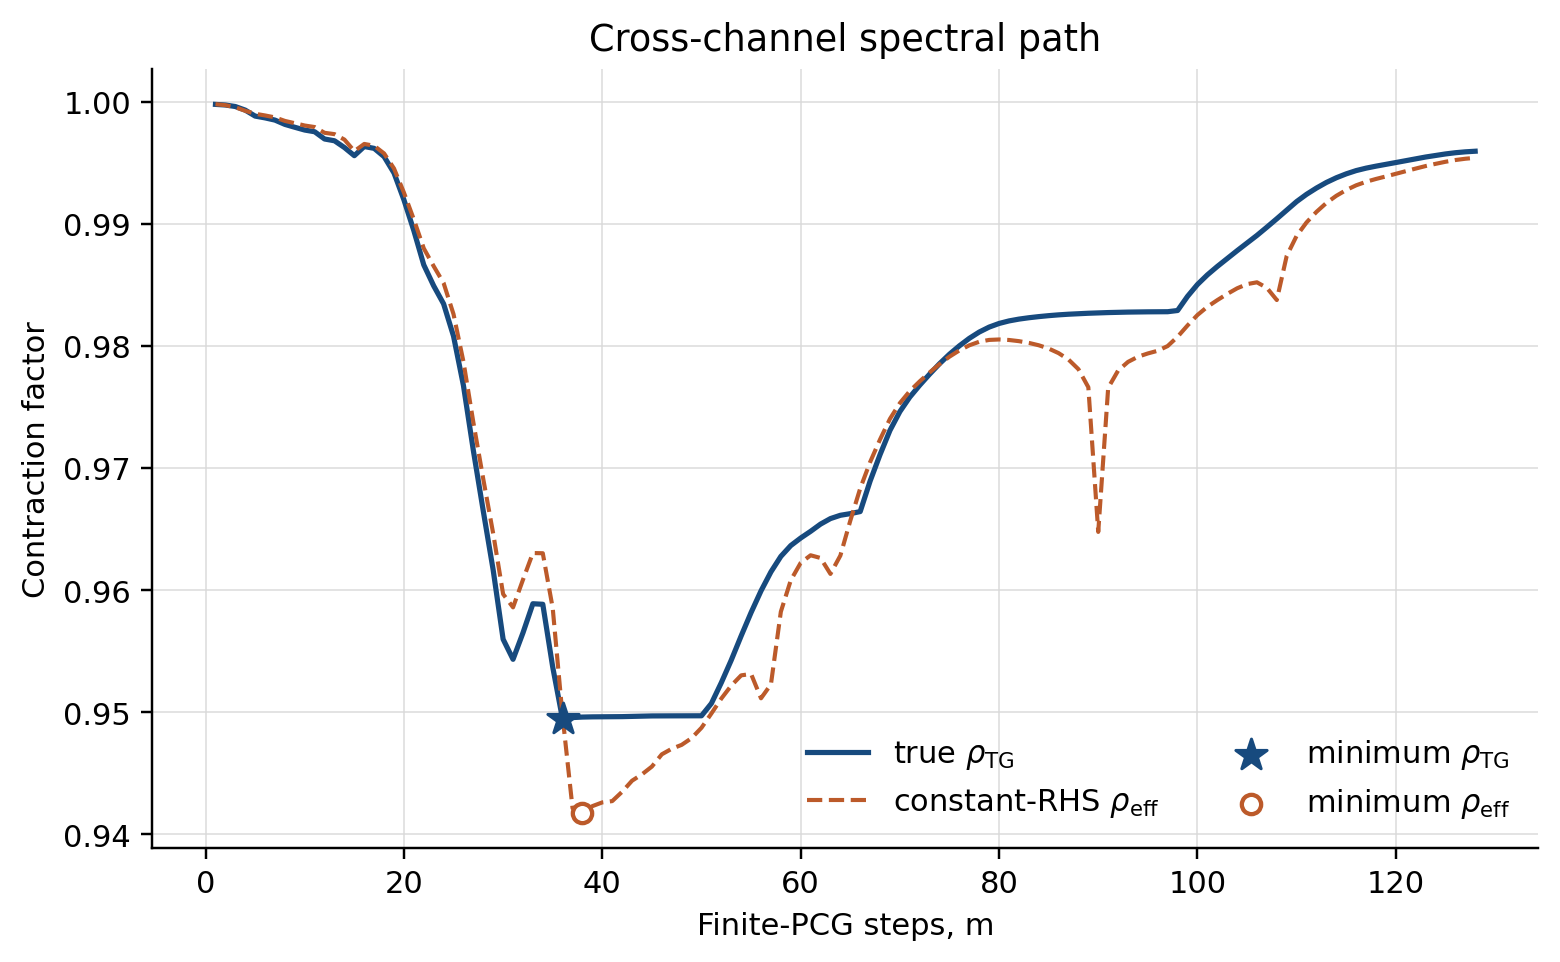
\includegraphics[width=.92\textwidth]{Fig1.png}
\caption{Cross-channel path: normalized energy decreases monotonically while the true two-grid spectral radius has a strict interior minimum.}\label{fig:cross-path}
\end{figure}
\begin{figure}[t]
\centering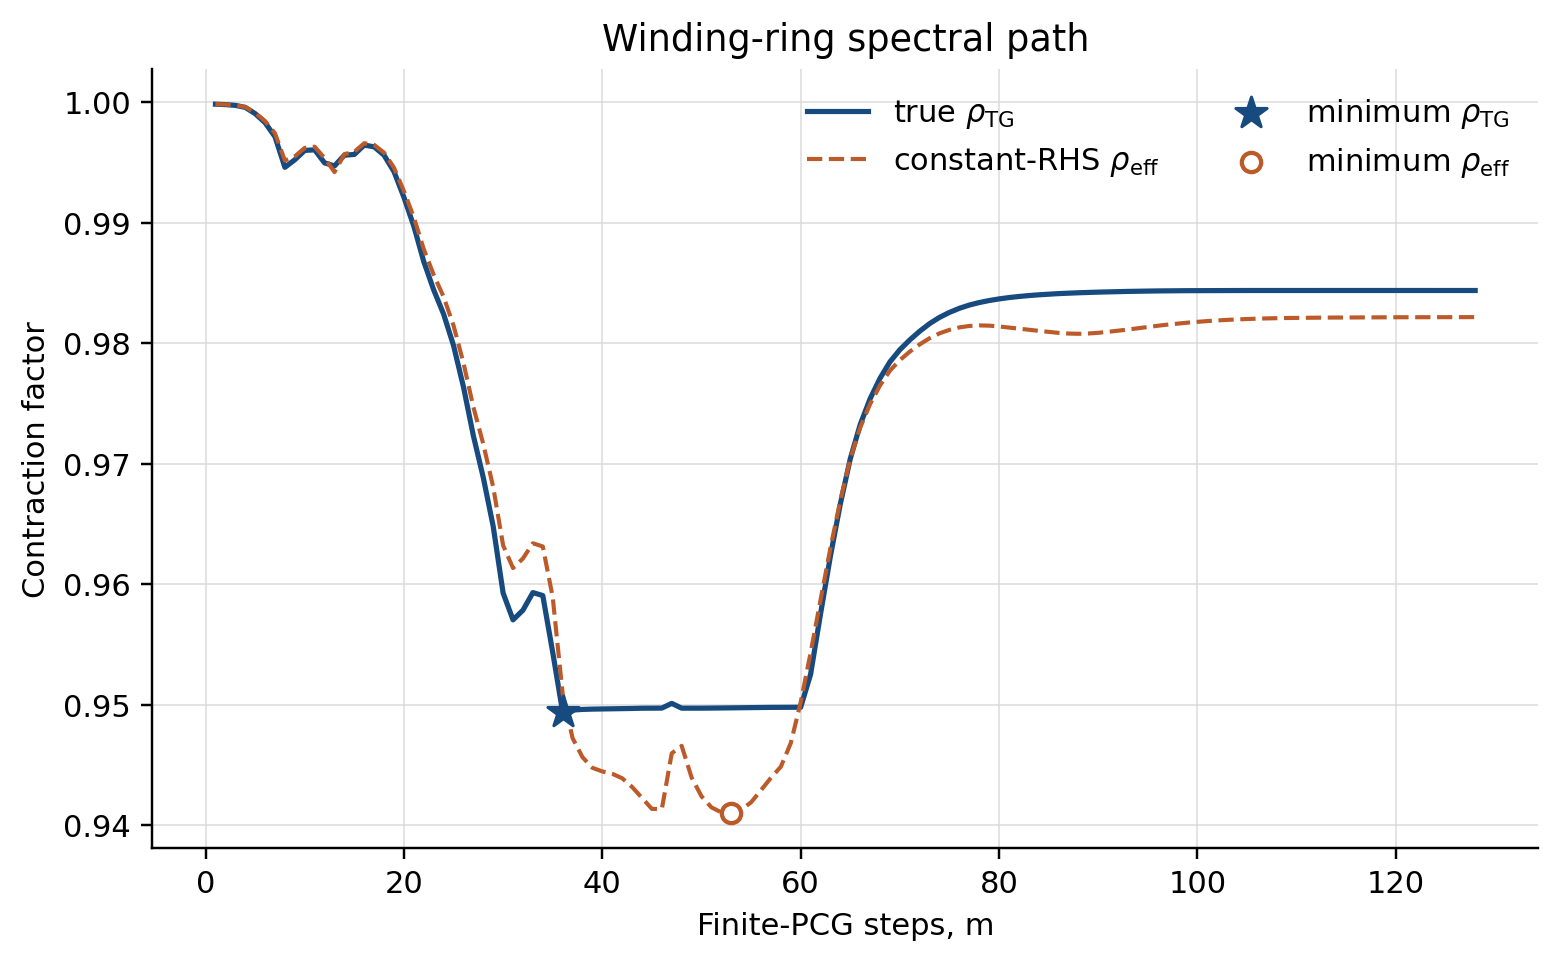
\includegraphics[width=.92\textwidth]{Fig2.png}
\caption{Winding-ring path. Nonmonotonicity persists under a distinct channel topology.}\label{fig:ring-path}
\end{figure}

\begin{table}[t]
\caption{Complete $128/16$, $\chi=10^4$ path scans.}\label{tab:path}
\centering
\small
\setlength{\tabcolsep}{3.5pt}
\begin{tabular}{lrrrrrr}
\toprule
Topology & $m_{\min\rho}$ & $\min\rho_{\rm TG}$ & $m_{\min\rm eff}$ & $\min\rho_{\rm eff}$ & endpoint $\rho_{\rm TG}$ & endpoint $\rho_{\rm eff}$\\
\midrule
cross &36&0.9494317&38&0.9417637&0.9961632&0.9957271\\
ring &36&0.9493862&53&0.9410121&0.9843675&0.9821588\\
\bottomrule
\end{tabular}
\end{table}

\subsection{Scaling, propagation, and the local theorem}
Two refinement families separate fixed $H$ from fixed $q=8$. The central-column correction satisfies the exact radius-$(m-1)$ propagation bound in all 16 full-run measurements, with zero violations at a $10^{-14}$ support threshold. Under fixed $H=1/8$, $m=q$ grows from 4 to 32 as $1/h$ grows from 32 to 256; the reached fraction remains near 19--22\%, consistent with the $\Theta(h^{-1})$ propagation scale. Under fixed $q=8$, the same $m=q$ remains eight and the reached fraction shrinks from 84.45\% to 1.26\%, matching the theoretical distinction in \eqref{eq:dichotomy}.

For a direct test of the local objects, a $16/4$ problem permits dense diagnostic export. At the endpoint,
$\sigma_1(T_F)=0.7896795471$, $\sigma_2(T_F)=0.7829979688$, and
$\delta=0.0066815783$. The endpoint construction defect is $3.44\times10^{-15}$, basis orthogonality defect is $1.28\times10^{-11}$, and the maximum discrepancy between the direct and graph formulas for $\rho_{\rm TG}$ is $4.07\times10^{-14}$. All 28 informative steps inside the certified local range have the sign predicted by the first-order direction; 42 of 52 informative steps agree over the wider diagnostic path.

\begin{figure}[t]
\centering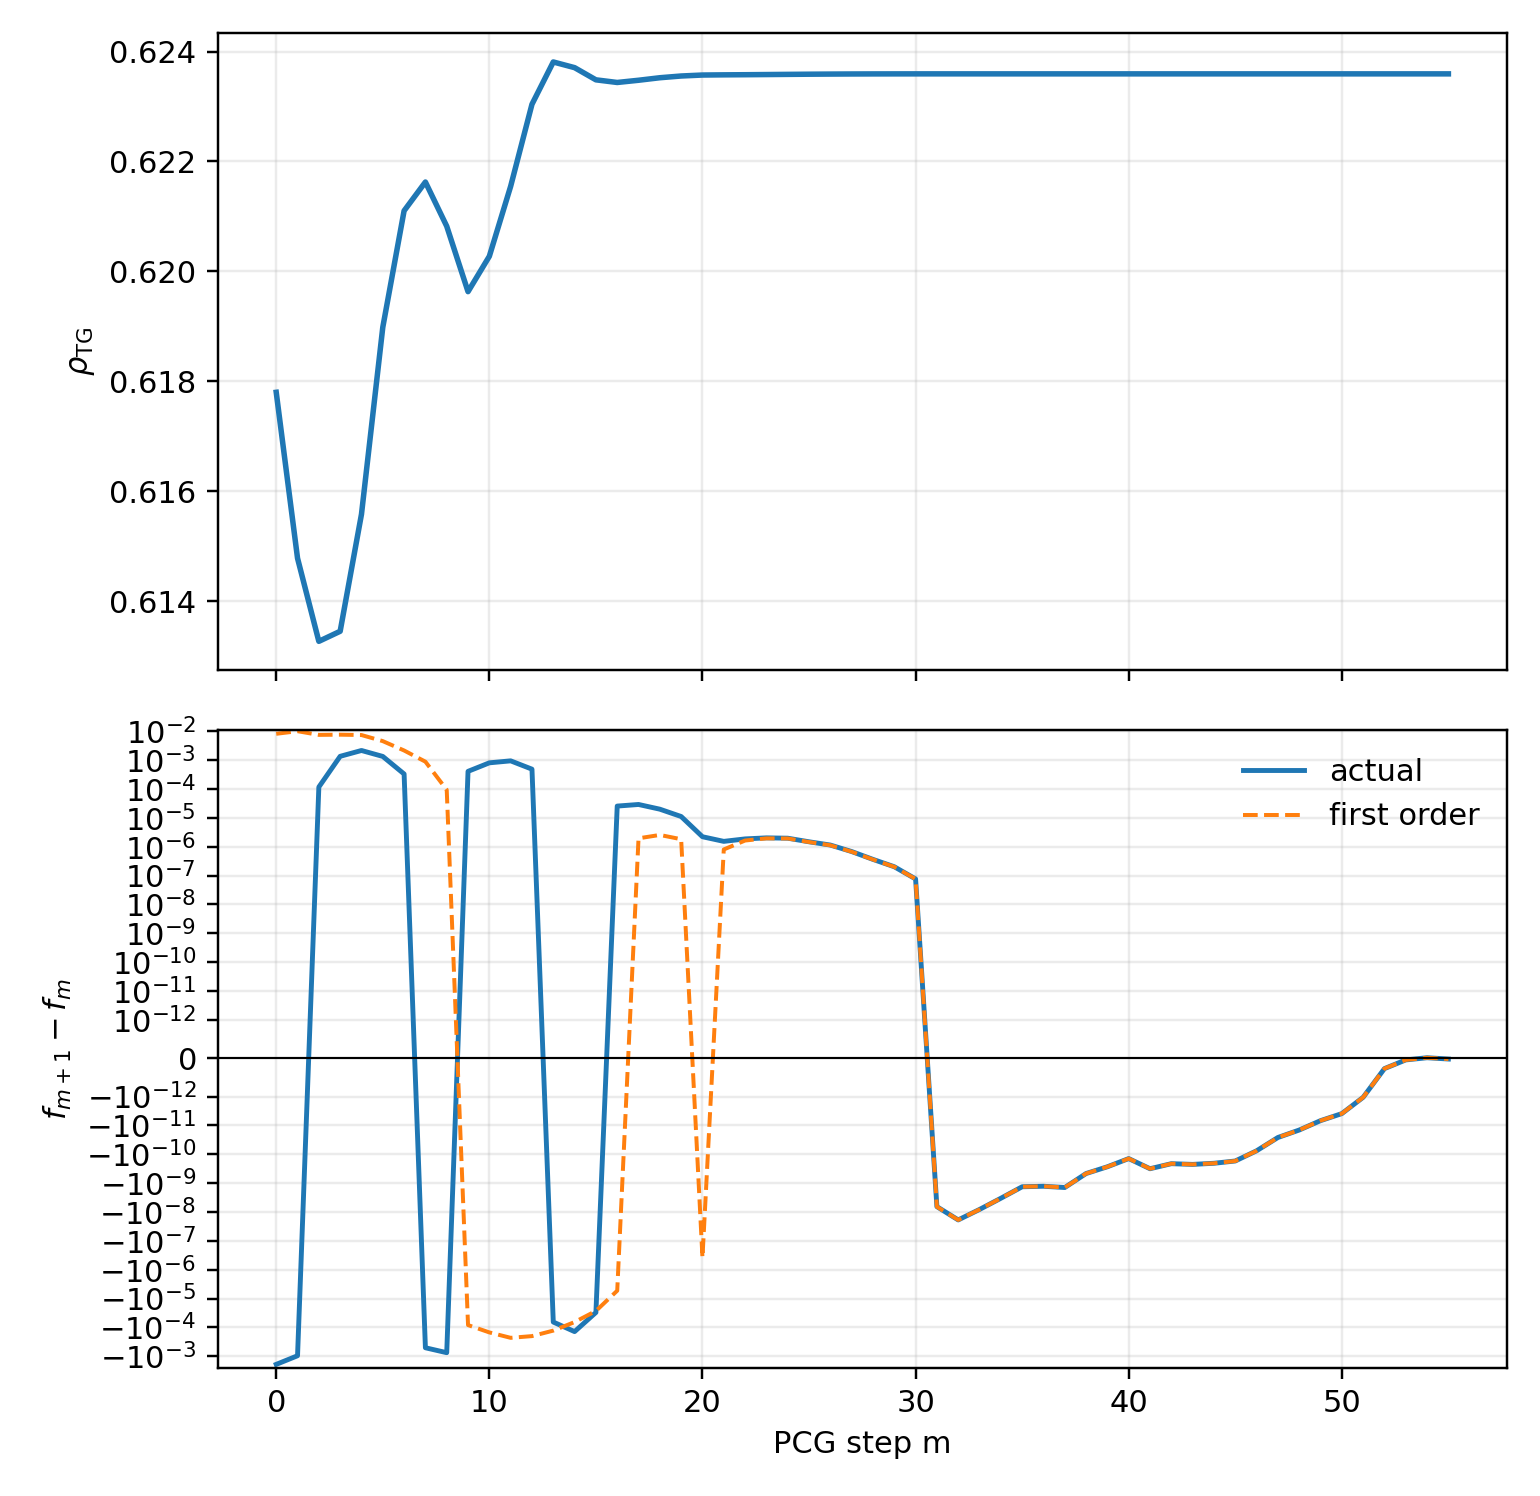
\includegraphics[width=.92\textwidth]{Fig3.png}
\caption{Local singular-gap diagnostic. The signed first-order quantity predicts the change of $\sqrt{\rho_{\rm TG}}$ throughout the certified local segment.}\label{fig:local}
\end{figure}

\subsection{Baselines, robustness, timing, and a multilevel pilot}
Table~\ref{tab:baseline} isolates the central problem. Energy minimization itself is highly beneficial, but finite PCG is substantially better and much sparser. Five coefficient seeds at $64/16$ give 327 total cycles for finite-$1/3$ and 866 for the endpoint; both methods converge in all cases. With the coefficient matrix and interpolation fixed and six qualitatively different right-hand sides, both methods again converge in all cases. Finite-$1/3$ uses 469 total cycles versus 1507 for the endpoint. One localized right-hand side favors the endpoint, which is natural because a single right-hand side need not excite the worst two-grid mode; the aggregate and worst-case outcomes favor the finite point.

\begin{table}[t]
\caption{Central $128/16$, $\chi=10^4$ cross-channel baseline.}\label{tab:baseline}
\centering
\begin{tabular}{lrrrr}
\toprule
Interpolation & Construction & Cycles & $\rho_{\rm eff}$ & density (\%)\\
\midrule
geometric & bilinear & 85524 &0.999838472&1.3950\\
energy endpoint & column relres $\le10^{-10}$ &3227&0.995727131&98.2099\\
finite PCG & $m=43$ &242&0.944406934&29.4678\\
\bottomrule
\end{tabular}
\end{table}

Five post-warmup timing repetitions alternate method order. Finite-$1/3$ averages 0.679 s total, compared with 10.193 s for the endpoint on the present machine, a factor of 15.01. The mean setup/solve split is 0.439/0.240 s for finite-$1/3$ and 2.553/7.640 s for the endpoint. The benefit therefore comes from both cheaper interpolation construction and a much faster solve. Since absolute timings are machine dependent, the repository records setup and solve components as well as deterministic cycle counts.

Finally, we apply the same construction independently on both Galerkin transitions of two three-level hierarchies. For $64/16/8$ cross-channel, finite-$1/3$ requires 70 V-cycles versus 321 for the endpoint; for $128/16/8$ winding-ring, the counts are 237 and 770. Replacing the exact coarse solve by one recursive V-cycle changes the corresponding exact-two-grid counts only from 65 to 70 and from 237 to 237 for finite PCG. These results show that the mechanism can survive one level of recursion, while a uniform multilevel theorem remains outside the present scope.

\section{Discussion}\label{sec:discussion}
The results refine the usual interpretation of iterative energy-minimizing interpolation in three ways.

First, the ideal or energy-minimizing endpoint is optimal for a precise interpolation functional, not for every solver objective. Equation \eqref{eq:exact-objective} makes the missing information explicit: the endpoint distance $\norm Z$ is insufficient without the orientation of $Z$ relative to $T_F$ and $T_*$. This is fully consistent with optimal-interpolation theory \cite{brannick2018optimal}; our contribution is to quantify the mismatch along the actual PCG construction path.

Second, truncation acts as a solver-aware regularization even though PCG itself only sees the energy equations. The effect is not a generic early-stopping slogan. It follows from the signed spectral weights in \eqref{eq:cross-weights}, is locally certified by Theorem~\ref{thm:step}, and is observed with the true two-grid spectral radius rather than only one residual history.

Third, the practically successful $O(h^{-1})$ budget is explained by propagation and conditioning under fixed physical coarse spacing. The capacity estimate also prevents overgeneralization: at fixed coarsening ratio the natural budget is $O(1)$ at bounded contrast. Thus the theory identifies which scaling regime is being exploited rather than treating $m\propto h^{-1}$ as a universal multigrid rule.

The present restrictions are transparent. We fix the coarse set, unit injection, one forward and one backward Gauss--Seidel sweep, and exact Galerkin coarse correction. The experiments use a structured two-dimensional diffusion operator. Constraint-preserving PCG, nonsymmetric smoothers, approximate coarse solves, unstructured discretizations, and fully recursive hierarchies require additional analysis. None of these limitations invalidates the central statement: within the standard controlled setting, the energy-minimizing endpoint can be dramatically inferior to an intermediate point on its own monotone construction path.

\section{Conclusion}\label{sec:conclusion}
Finite Jacobi--PCG iterates should be viewed as a family of coarse spaces, not merely inaccurate approximations to ideal interpolation. The normalized graph coordinate gives an exact bridge from interpolation energy to coarse-space angles and the true two-grid spectral radius. It proves why strict energy decrease can coexist with either improvement or deterioration of two-grid convergence, and it produces explicit local and pathwise certificates. The sharp two-dimensional capacity scale explains the finite iteration budgets observed under aggressive coarsening. Across difficult high-contrast experiments, the finite path is simultaneously sparser, cheaper to construct, and substantially faster to solve with than the high-accuracy energy endpoint. This establishes a robust and practically meaningful mechanism for linear systems in which coefficient contrast and unresolved or barely resolved microstructure make conventional interpolation ineffective.

\begin{acknowledgements}
The author information, funding statement, and acknowledgements will be completed before submission.
\end{acknowledgements}

\section*{Declarations}
\textbf{Conflict of interest.} The author declares no conflict of interest.\par
\textbf{Data and code availability.} Source code, scripts, numerical data, and the manuscript source are provided in the accompanying reproducibility archive and at the project repository. The public repository URL will be updated to the archival v10.0 release before submission.\par
\textbf{Author contributions.} The named author is responsible for the mathematical analysis, software, numerical experiments, interpretation, and manuscript.

\appendix
\section{A singular-value perturbation estimate}\label{app:sv}
For completeness, we state the perturbation result used in Theorem~\ref{thm:expansion}. Let $\sigma_1(M)-\sigma_2(M)=\delta>0$ and let $u,v$ be leading singular vectors. If $e=\norm E_2<\delta/2$, then
\begin{equation}\label{eq:sv-app}
 \abs{\sigma_1(M+E)-\sigma_1(M)-u^{\T}Ev}
 \le\frac{e^2}{\sqrt{\delta(\delta-2e)}}.
\end{equation}
To prove it, form the symmetric dilation
$\mathcal M=\left[\begin{smallmatrix}0&M\\M^\T&0\end{smallmatrix}\right]$ and its perturbation $\mathcal E$. The leading eigenvalue of $\mathcal M$ is simple and has gap at least $\delta$. Resolve the perturbed normalized eigenvector into its leading component and orthogonal complement. The orthogonal equation and the spectral gap give
$\sin\vartheta\le e/(\delta-e)$. Substitution into the leading scalar equation, followed by the sharper normalization identity
$1-\cos\vartheta=\sin^2\vartheta/(1+\cos\vartheta)$, yields \eqref{eq:sv-app}. The dilation vectors contribute the same first-order scalar $u^{\T}Ev$.

\section{Reproducibility map}\label{app:repro}
The archive separates deterministic mathematical quantities from machine-dependent timing.
\begin{itemize}
\item Experiment 1 generates all 13 finite-checkpoint/endpoint comparisons and aggregate densities.
\item Experiment 2 generates both complete spectral paths and their figures.
\item Experiment 3 generates fixed-$H$/fixed-$q$ scaling and verifies finite propagation.
\item Experiment 4 exports the small dense matrices used to independently reconstruct $Z,T_F,T_*$ and the local sign diagnostic.
\item Experiment 5 tests coefficient seeds, six fixed-interpolation right-hand sides, and alternating-order repeated timings.
\item Experiment 6 isolates geometric versus energy-minimizing interpolation.
\item Experiment 7 is the three-level V-cycle feasibility study.
\end{itemize}
The run script rebuilds every executable in release mode, overwrites the formal result files, and regenerates all three figures. No precomputed matrix is required.

\bibliographystyle{spmpsci}
\bibliography{references}
\end{document}
